% !TeX root = ntfs.tex
\section{Addressing Storage: Clustering}
\label{sec:Cluster}
Before we can begin to organize files, we first need to be able to manage the available space. In order to divide up the storage medium NTFS has devised a system called Clustering.

The basic idea of clustering is to divide up the storage medium into contiguous parts, called \textit{clusters}. These clusters are made up of $2^n, n \in \mathbb{N}$\cite{microsoftinc:2018:DCS} sectors (areas usually sized $512$ Bytes) on a storage device and hence abstract from the physical layout. When formatting a volume the size of clusters can be set, but it cannot be changed afterwards (without formatting again).\\
 %TODO: Add citations
Setting the cluster size seems at first glance like an arbitrary choice of size, but it is not. It is a trade-off between internal fragmentation and speed:
When increasing the cluster size there is less management overhead for the clusters as there is fewer of them. The reduced overhead will improve speed.\cite{RUSSINOVICH_ET_AL:2012:WI} Further due to the clusters being mapped to contiguous blocks the speed of access is also improved with larger cluster sizes, as especially for media with mechanical parts accessing contiguous memory is a lot faster due to less mechanical movement required. As for solid state memory contiguous access still provides speed benefits, as SSDs do not load one block at a time but rather a collection of consecutive blocks at the same time.\cite{BELLOSA:2017:OS}
At the same time though, when larger cluster sizes are set there is potential for clusters only partially containing actual data and hence potential for a less efficient use of the available storage space. The latter problem is called internal fragmentation.  
In figures \ref{fig:internal_frag_16} and \ref{fig:internal_frag_4} this is illustrated. In this example we are storing 2 KiB of data in a cluster. With the cluster size set to 4 KiB (figure \ref{fig:internal_frag_4}) we can see that we have less space that cannot be used due to our memory allocation compared to the cluster size set to 16 KiB (figure \ref{fig:internal_frag_16}). Specifically when using the 4 KiB clusters we lose $50\%$ of the allocated storage to internal fragmentation, whereas for the 16 KiB clusters we lose $87.5\%$.
\begin{figure}[H]
	\centering
	\fbox{
		\resizebox {0.95\columnwidth} {!} {
			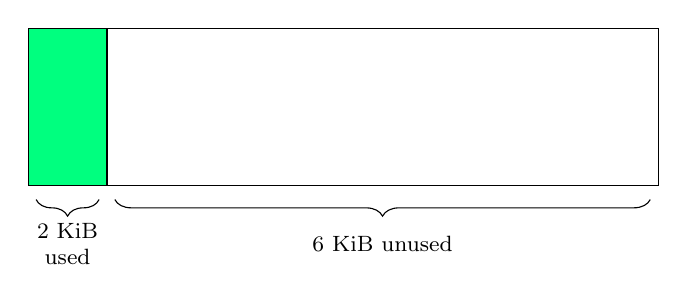
\begin{tikzpicture}[scale=1]
				\filldraw [fill=SpringGreen, draw=black] (0,0) rectangle +(1,2);
				\filldraw [fill=white, draw=black] (1,0) rectangle +(7,2);
				\draw [decorate,decoration={brace,amplitude=6pt,mirror,raise=1pt},xshift=0pt,yshift=-4pt,font=\footnotesize,align=center]
				(0.1,0) -- (0.9,0) node [black,midway,yshift=-0.6cm]
				{$2$ KiB\\used};
				\draw [decorate,decoration={brace,amplitude=6pt,mirror,raise=1pt},xshift=0pt,yshift=-4pt,font=\footnotesize,align=center]
				(1.1,0) -- (7.9,0) node [black,midway,yshift=-0.6cm] 
				{$6$ KiB unused};
			\end{tikzpicture}
		}
	}
	\caption{Illustration of internal fragmentation: Cluster size 16 KiB\label{fig:internal_frag_16}}
\end{figure}
\begin{figure}[H]
	\centering
	\fbox{
		\resizebox {0.95\columnwidth} {!} {
			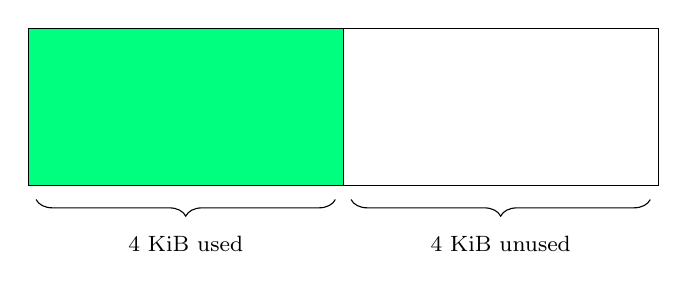
\begin{tikzpicture}[scale=1]
				\filldraw [fill=SpringGreen, draw=black] (0,0) rectangle +(4,2);
				\filldraw [fill=white, draw=black] (4,0) rectangle +(4,2);
				\draw [decorate,decoration={brace,amplitude=6pt,mirror,raise=1pt},xshift=0pt,yshift=-4pt,font=\footnotesize,align=center]
				(0.1,0) -- (3.9,0) node [black,midway,yshift=-0.6cm]
				{$4$ KiB used};
				\draw [decorate,decoration={brace,amplitude=6pt,mirror,raise=1pt},xshift=0pt,yshift=-4pt,font=\footnotesize,align=center]
				(4.1,0) -- (7.9,0) node [black,midway,yshift=-0.6cm] 
				{$4$ KiB unused};
			\end{tikzpicture}
		}
	}
	\caption{Illustration of internal fragmentation: Cluster size 4 KiB\label{fig:internal_frag_4}}
\end{figure}
By default Microsoft has set the cluster size for usual desktop storage capacities (2GB - 16TB) to $4$ KiB \cite{microsoftinc:2018:DCS}. For larger storage needs the default cluster size is $>4$ KiB, as one would usually not worry about internal fragmentation that much, but having faster access speeds is very important.

\subsection{Virtual and Logical Clusters}
\label{sec:Cluster:CN}
Now that we have established that clusters are just some unit of memory that addressed lets look at how the addressing works. \\
For this we will now need to distinguish between Logical and Virtual clusters:
\begin{itemize}
	\item Logical clusters are the physical collections of sectors on a disk 
	\item Virtual clusters are the clusters that are used within a given file
\end{itemize}
So the name space of virtual clusters is file local, whereas the name space of logical clusters is global. 
All used virtual clusters in a file are mapped to logical clusters. Virtual clusters which lack any meaningful, i.e. there is only zeros stored in them,  are not mapped to logical clusters. 
%TODO: Go deeper!
This allows for sparse files, i.e. files that are mostly empty, to not occupy a lot of disk space, as the disk space would not actually store any proper data.\\
Going back to addressing: Virtual clusters are referenced by Virtual Cluster Numbers (VCNs). The first VCN of a file always has an index of $0$ and every other VCN indicates the offset from the beginning of the file. This can be expressed as the following invariant:
\begin{center}
\texttt{A VCN with value $n$ represents the $(n+1)$\textsuperscript{th} cluster in a file}\\
\end{center}
Logical Cluster Numbers (LCNs) on the other hand are indices for logical clusters and represent the offset from a given (arbitrary, but constant) point on the medium, which has been assigned LCN $0$.\cite{RUSSINOVICH_ET_AL:2012:WI}